\documentclass[a4paper, 10pt, twocolumn]{article}

\usepackage{graphicx}                % optional für Grafiken
\usepackage[font=footnotesize]{caption}
\usepackage[section]{placeins}
%\usepackage{tabularx}               % optional für Tabellen
%\usepackage{multirow}               % optional für Tabellen
\usepackage{url}                	 % optional für Internet Links
\usepackage{hyperref}

%\usepackage[small,bf]{caption3}     % Bildunterschriften

%\usepackage{parskip}

% verbatim with line line wrapping
% \usepackage{listings}
% \lstset{
%    breaklines=true,
%    basicstyle=\ttfamily}

\usepackage{titlesec}
\usepackage{amsmath}                
\usepackage{amssymb}
\usepackage{abstract}

% temporal packages
\usepackage{lipsum}
\SetLipsumDefault{1}

%\usepackage{enumitem}
%\setlist{nosep} % or \setlist{noitemsep} to leave space around whole list

\usepackage{xcolor}
\newcommand{\highlight}[1]{\colorbox{yellow}{\parbox{\columnwidth}{#1}}}

%\pagestyle{empty}                   % weder Kopf- noch Fußzeile auf 1. Seite
\graphicspath{{figures/}}


\begin{document}

\date{\small\today}                                        % kein Datum auf 1. Seite
\title{
	\vspace{-20mm}\textbf{	\large 
	Plankton Retention mechanism studies at Elbe with IBM}
	}
\author{
	Laurin Steidle\(^1\), Ross Vennel, Jana Hinners \\
	\emph{
		\small
		\(^1\)laurin.steidle@uni-hamburg.de} \\
	\emph{
		\small Universitaet Hamburg, Grosse Elbstrasse 133, Germany}
		}

%--------------------------------------Abstract------------------------------------------------

\twocolumn[
	\begin{@twocolumnfalse}
		\maketitle

		\begin{abstract}
			\begin{center}
				\texttt{All texts in this typewriter fond are drafting comments and thoughts on the text itself and not part of the actual paper.}
				\smallskip
			\end{center}
			
			\begin{center}
				\texttt{placeholder abstract - not to be proofread}
				\smallskip
			\end{center}

			% \begin{figure}
			% 	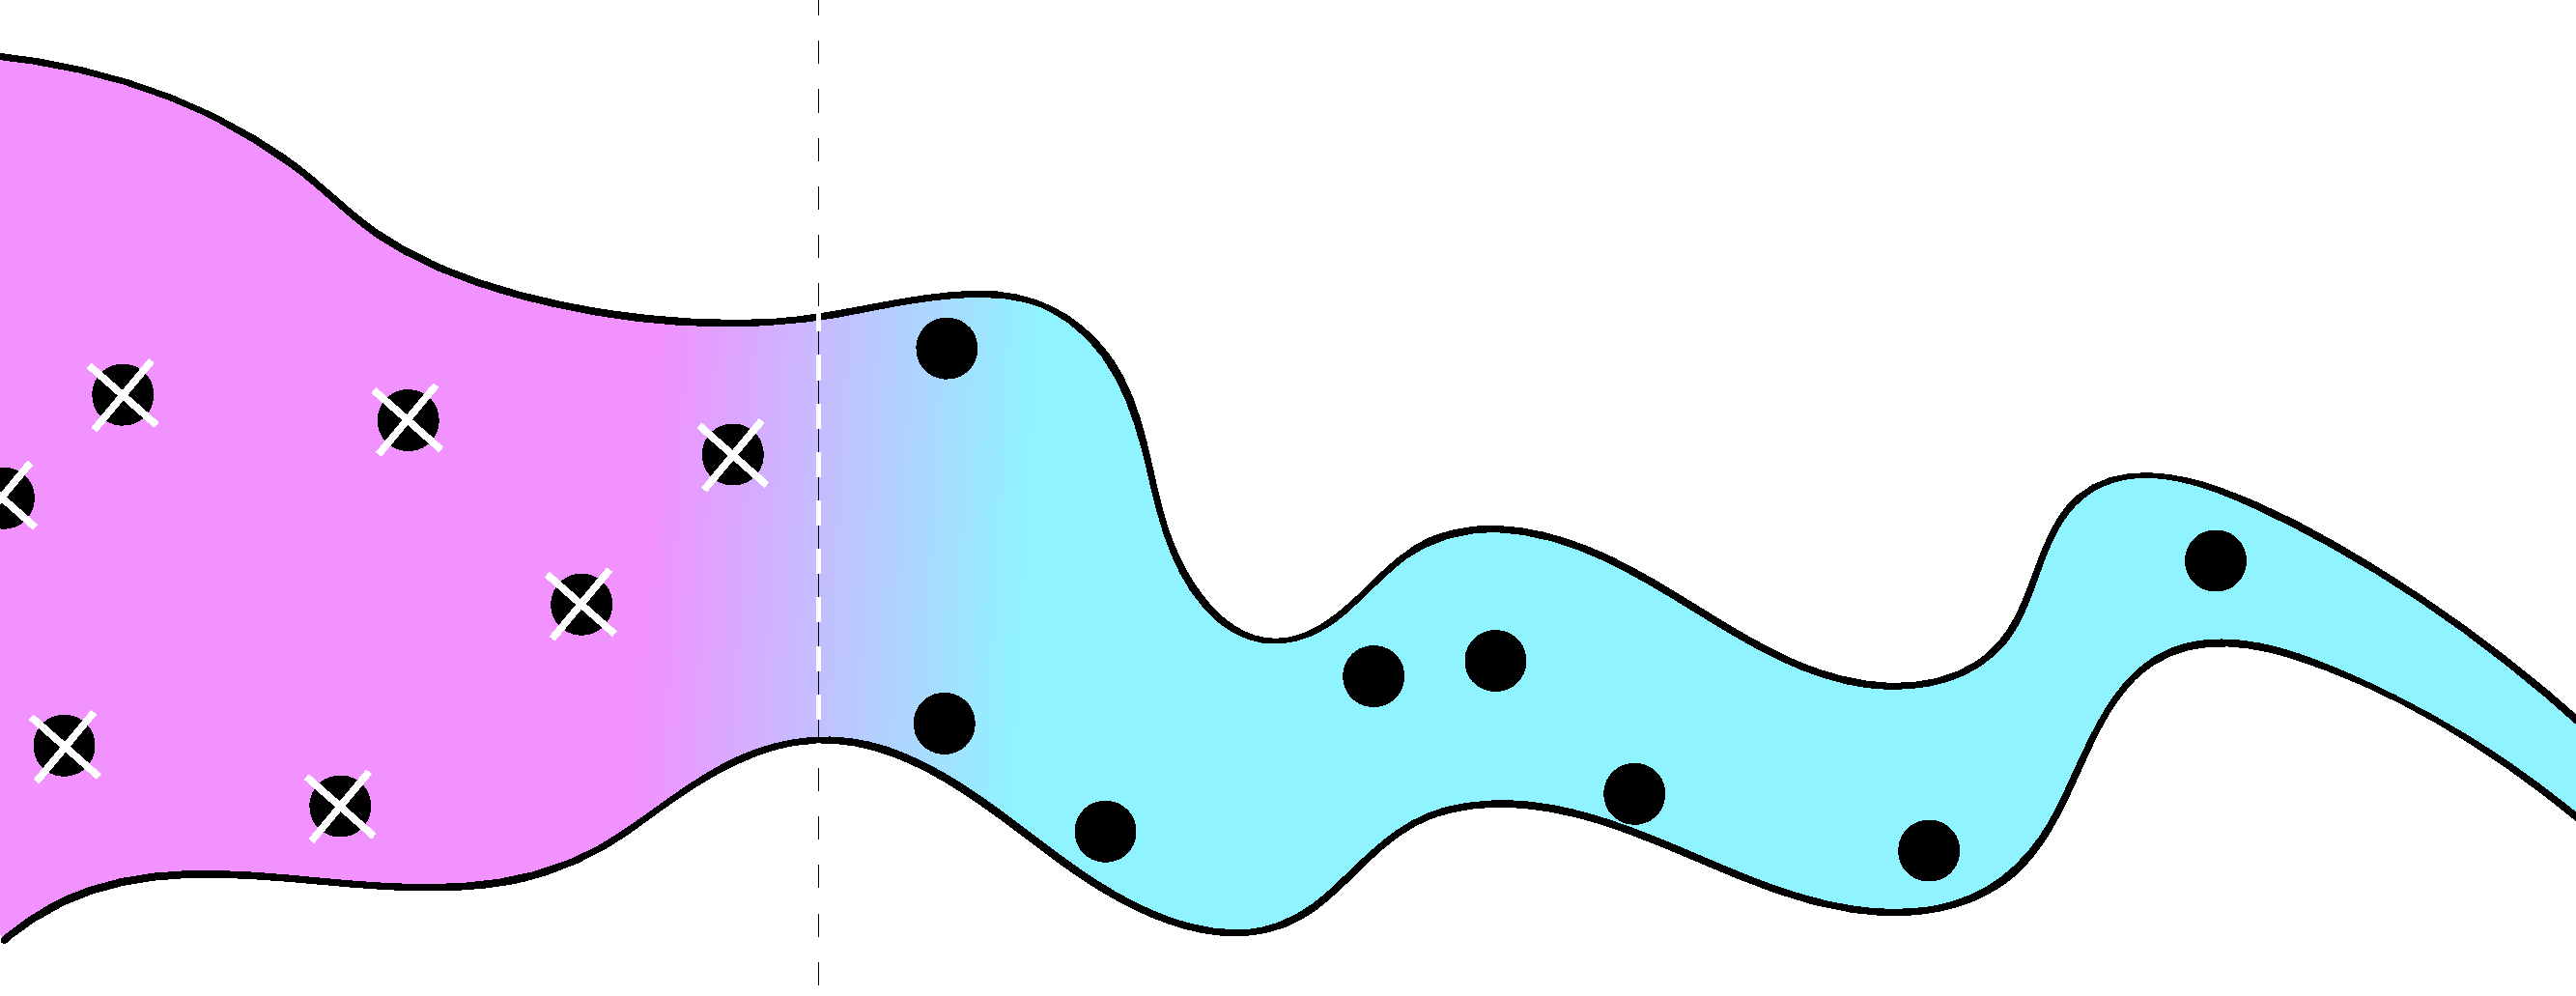
\includegraphics[width=\columnwidth]{picto visual abstract.pdf}
			% \end{figure}
			Estuaries are a challenging environment for plankton.
			Gradients are steep and currents are strong.
			Retention mechanisms are crucial for their survival.
			However, very little experimental and theoretical evidence has been gathered on the mechanism of phytoplankton retention.
			We will conduct a model study.
			First we will show the importance of retention mechanism for plankton in the Elbe.
			Secondly we will study different retention mechanism and comment on their importance.
			\vspace{1cm}
		\end{abstract}
  	\end{@twocolumnfalse}
]


\section*{Introduction}


\subsection*{Estuaries and Phytoplankton}

\textbf{Estuaries are important} both for the climate system as well as for anthropogenic use.
From a climate perspective they offer a high productivity relative to surface area which results in large amounts of direct carbon cycling as well as their important role as a source of nutrients and hatching grounds for marine ecosystem. (cite)
They are also strongly anthropogenically influenced through e.g. harbors, diking and fishing which can be seen as a stressor on the ecosystem but also adds am anthropogenic dependency on the well being of the ecosystem.

However, estuaries are also complex and strongly dynamic ecosystem such that it is still difficult to predict ecosystem dynamics or the effects of anthropogenic changes to this day.
This complexity arises from the topology and the resulting hydrodynmics at the fresh-salt water interface.

As for most ecosystem - their dynamics are strongly controlled by the primary producers.
However phytoplankton, the major aquatic primary producer drifts in the current as all planktonic organism.
Due to the current in the estuary we expect plankton to be drifting downstream over time and ultimately be washed out into marine high salinity waters.
Hence, we wonder how phytoplankton manages to survive as a populating in such an environment.
If we assume that the population is not exclusively maintained by upstream plankton that is washed into the estuary
 then there must be some sort of retention mechanism that enables a phytoplankton population to not be washed out.
While this is expected to be an crucial mechanism for survival  it is currently not well understood 
due to the difficulty in either measuring or modeling such processes.



\subsection*{what is known}


We categorize the already performed studies on the subject of phytoplankton retention in three groups: observations, theoretical- and realistic-modelling studies.

\textbf{Observational} studies have found three major mechanism for retention - diel migration, sinking and stickiness.
Diel migration (moving verticaly up and down with the sun) has been found but so far only shown for larger estuarine organisms which are not strictly planktonic i.e. zooplankton [cite]
Also benthic plankton has been observed to be strongly negatively buoyant, hence sinking and sticking to the ground.

Next want to highlight two more \textbf{theoretical} studies studying the mechanisms of "loss compensation" and "reseeding".
(cite) theorized a set up in which they  a population is able to maintain itself if the losses due to outwashing can be compensated by growth (cite).
In a setup where a lagoon like ecosystem was modelled they were able to quantify reproduction thresholds that are needed to maintain the population.
However, this setup also implies that the growing part of the population is somehow retaining their position.
If the regrowing population is also continuously drifting downstream they will also ultimately die out.

(cite) studied the concept of "reseeding".
Here a system is theorized in which a population is able to repopulate an previously 
uncolonized area upstream due to local upstream currents e.g. through larger eddies.
While they showed that upstream reseeding is conceptually possible they did so in a special contrived system.
Whether this is an actual realized phenomenon depends on the topology and hydrodynamic of the estuary.

\smallskip
\texttt{More detail?}
\smallskip

Hence, it has been showed both "outgrowing the losses" and "reseeding" are possible retention mechanism but only under certain conditions.



In (cite) they use a \textbf{particle tracking model} also known as Lagragian model to study Zooplankton movement in the San Francisco Bay.
They were able to show  that sinking and diel migration slows the outwashing process and might be beneficial retention tactic.
However, they did so by ignoring key processes like reproduction and death in an rectangular grid model
which further introduces some numerical artefact.


To \textbf{summarize} - several concepts for potential retention mechanisms have been found
 and shown to work in certain conditions.
However, all approaches used major simplification which didn't allow them to study the full picture.
We developed a new and more realistic approach to study retention with an particle tracking model combining
 many of the above outlined features into one model.

\texttt{I don't have a proper "thats our hypothesis" part in my introduction which is considered to be bad style I think.
        However, the way I frame it currently I don't really have a proper hypothesis. 
        I approached it more as a kind of "lets see if we can find some noteworthy patterns and report them"
        Personally I think this kind of playing around is worth communicating as well but I am not sure how the community feels about that.}

\section*{Methods}

\subsection*{general model description}

In our study we take a particle tracking approach with a \textbf{lagrangian model} called Oceantracker (cite).
Particle tracking offers several advantages for our question:
While particle tracking on unstructured grids has been relatively computationally expensive until recently (cite)
 it allows us to reuse already validated hydrodynamic models.
Reusing already computed and calibrated hydrodynamical models is overall much faster then solving the advection-diffusion again.

Additionally, because we are tracking particles individually we are able to observer their individual tracks.
This makes it much easier and intuitive to interpret the results and allows us to  include "individual based processes".

\texttt{better representation of the particle behavior close to the edges of the estuary?}

\begin{figure}
    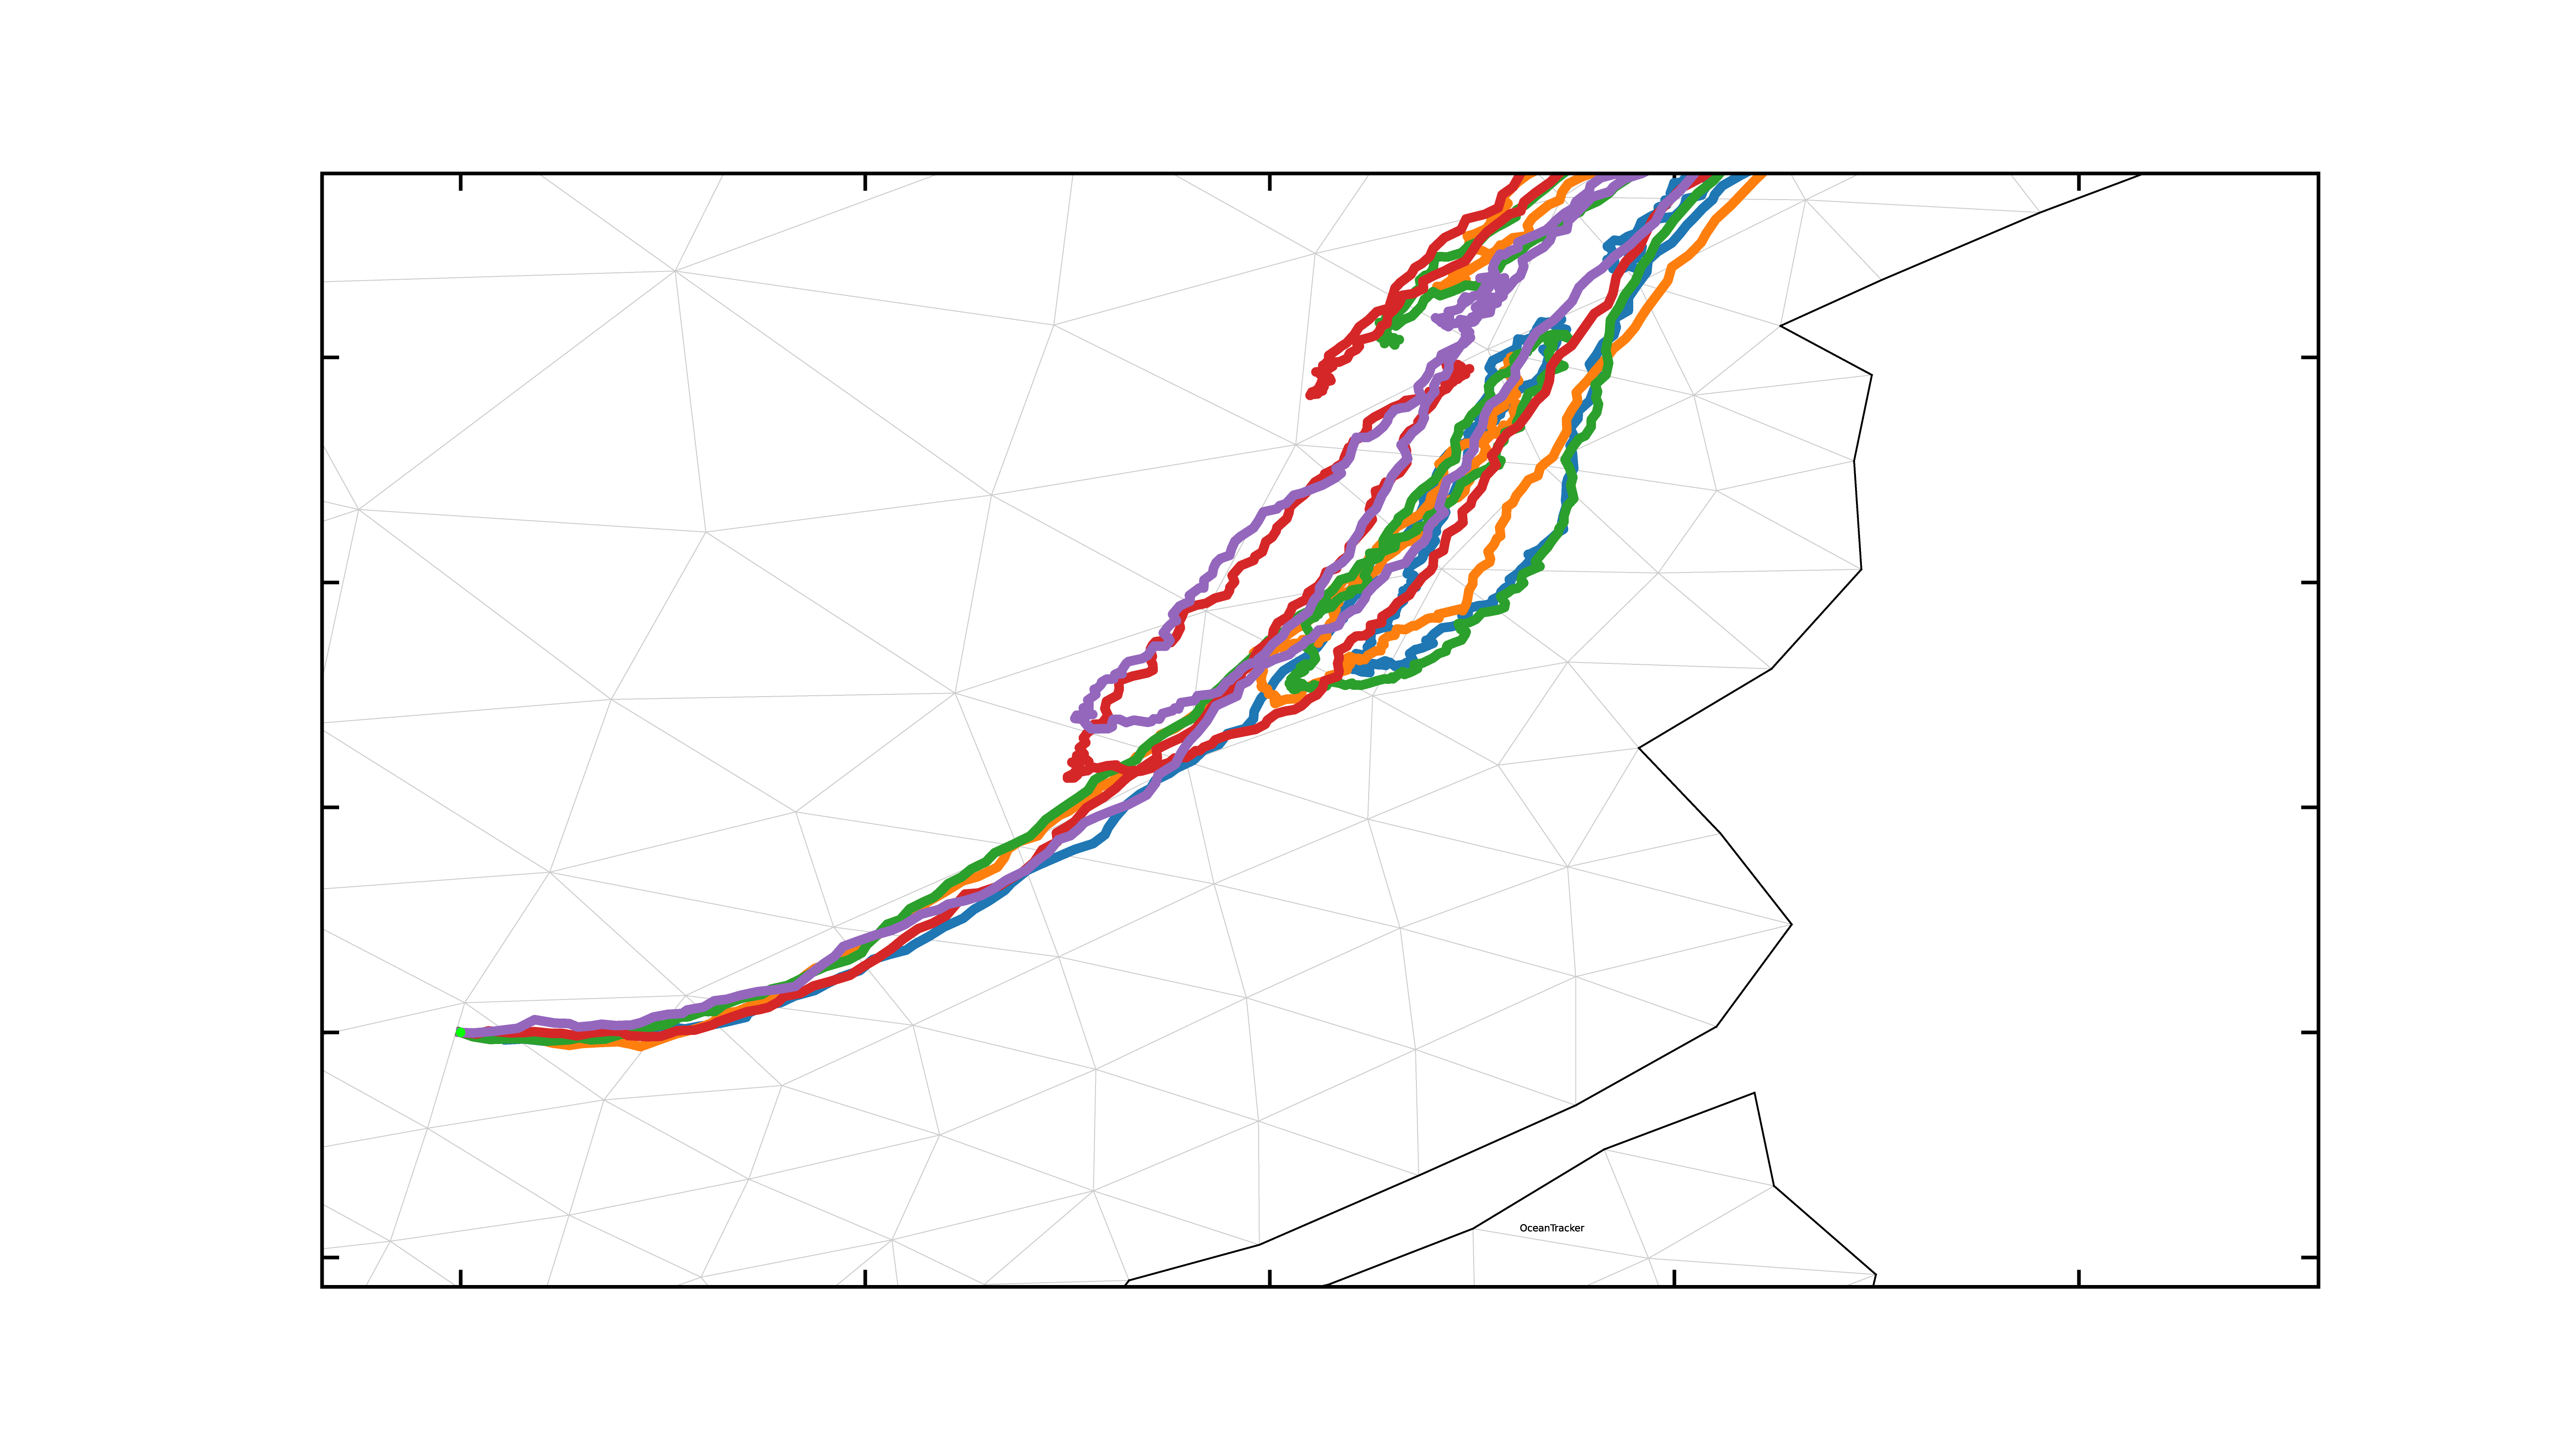
\includegraphics[width=\columnwidth]{Artboard 2.png}
    \caption{Particle Trackle visualisation - particle tracks on grid}
\end{figure}

The hydrodynamics \textbf{data} is taken from a SCHISM model from a Johannes Pein (cite).
It is an three dimensional unstructured  grid model representing the full Elbe estuary from the weir at Geesthacht close to helgoland including side-channels and the harbor area.
% (Look for more details in pein paper that might be interesting)
It provides a node-based mesh field containing a range of information.
For our purpose the water velocities represented in a flow field is the most important one
But also salinity and many other more technical information is used (See appendix \texttt{not yet added})
We study the year 2012 with 1h temporal- and dynamically varying spacial resolution.

\begin{figure}
    \includegraphics[width=\columnwidth]{dfg_foto_wettbewerbg_laurin_legendless_steidle.png}
    \caption{model domain visualization - full range grid including statistical polygons for later reference and example of a scalar field (e.g. temperature)}
    \label{fig:statistial polygons}
\end{figure}

On top of the "blanc" particle we add a set of textbf{biological features} to achieve a more realistic behavior.
The most important one is their ability to reproduce by creating copies of themselves 
and their ability to die in certain conditions.
We also add a set of movement related features. 
This includes a vertical movement behavior. 
We included constant vertical velocities i.e. sinking and rising and a time dependent one namely diel-migration.
Their interaction with the boundaries of our model is represented by a simple sedimentation and resuspension model in the water and in a stranding model on land

% \begin{figure}
%     \centering
%     \begin{minipage}{.4\columnwidth}
%         \centering
%         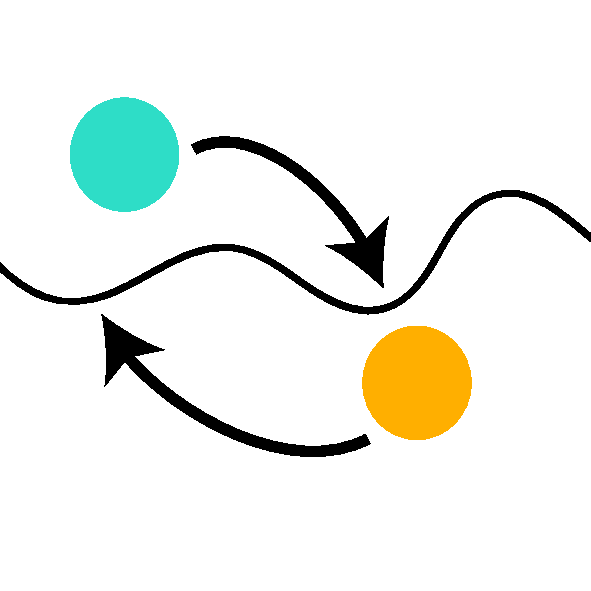
\includegraphics[width=.3\columnwidth]{picto resuspension.pdf}
%     \end{minipage}
%     \begin{minipage}{.4\columnwidth}
%     \centering
%         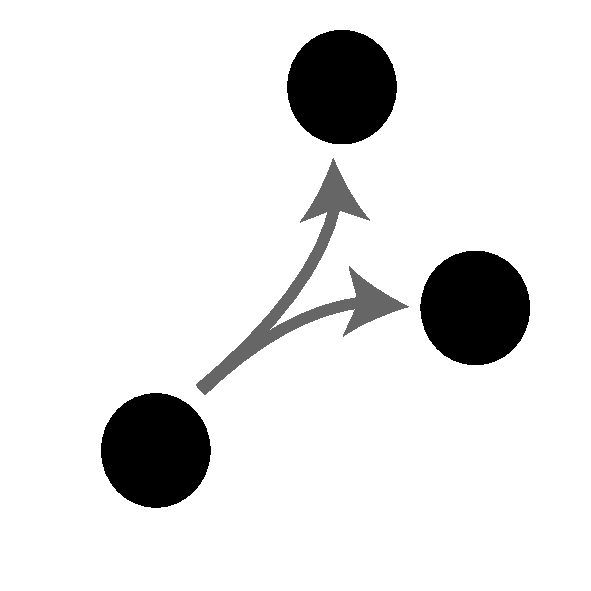
\includegraphics[width=.3\columnwidth]{picto splitting.pdf}
%     \end{minipage}
%     \caption{examples of pictograms for bio processes}
% \end{figure}



% \begin{figure}
%     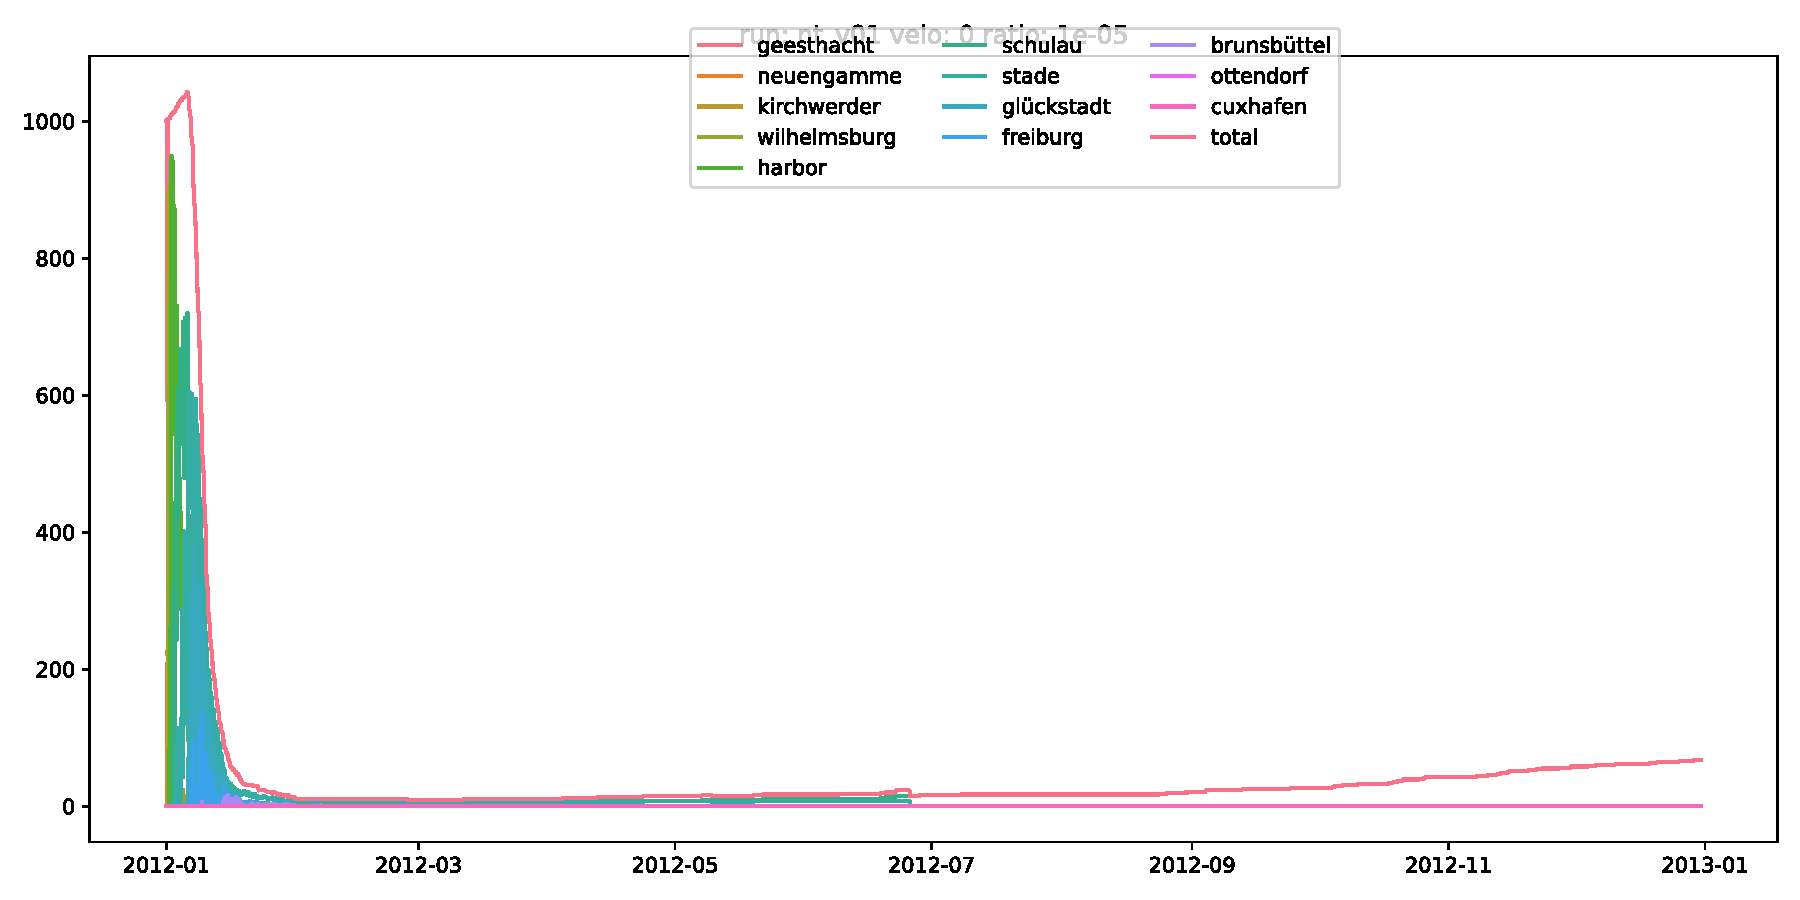
\includegraphics[width=\columnwidth]{fixed_particle_culling.pdf}
%     \caption{Example 2d plot of particle counts, centroid and "retainment" threshold}
% \end{figure}

\subsection*{Experimental configurations}

% \begin{figure}
%     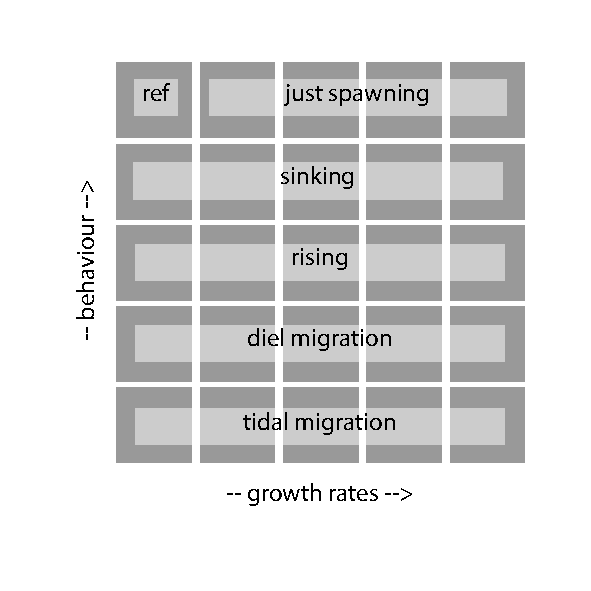
\includegraphics[width=\columnwidth]{plot experimental configuration.pdf}
%     \caption{2d grid with boxes for the different cases/dimension. 
%              Same structure as the later sensitivity analysis plot used \ref{fig:retention_results_SA}}
%     \label{fig:experimental_configuration}
% \end{figure}


\textbf{downstream retention}
The first and major experiment of this studies examines retention mechanisms under different scenarios.
General idea is to release a population of plankton at the beginning of the estuary represented by the weir in Geesthacht 
and examine how the population distrubutes itself over the estuary and whether it is able to maintain its population size.
With this approach we study the effect of several mechanism. These include:
\textit{Reproduction} represented as a chance of duplicating a particle,
\textit{vertical migration} where two modes have been implemented. 
A constant up or downward drift and diel migration where the drift speed and direction is based on the phase of the sun.
The particle \textit{stranding and resuspension} as well as \textit{suspend and resuspension to and from the bottom}
 based on a critical-friction-velocity model.
Particles are removed if they either reach high salinity waters implemented as a mortality chance above $10 PSU$,
when they are stranded until they dry out which is represented by killing all particles which have not been rewettet
 in the last $7$ days, and when they are starved for light which we defined as removing all particles which have been
 in low-light areas longer then a total of $14$ days where presence in high-light areas is subtracted from the starvation budget.
\texttt{Sentences to long to assume - good enough for now}
The model also implements dynamic dispersion that is crucial to represent tidal-pumping processes 
and to allow for a realistic trajectories close to boundaries.

\smallskip
\texttt{More detail needed? - or should that go into the appendix?}
\smallskip

The observed particle batch representing our phytoplankton population is released at new years eve in a volume at the weir in Geesthacht which marks the beginning of the Estuary.
We evaluate their \textbf{retention success} primarily by measuring the amount of plankton in different regions in the estuary over time.
If the population survives a full year and its population is over a certain threshold we consider them "successfully retained".

To count the particles we use "\textbf{statistical polygons}" that split the estuaries in along-shore sections. 
See  \ref{fig:statistial polygons}.
We also log their distance traveled, age, water depth, and status - whether they are drifting, stranded on the shore or bottom.
This allows us to compare the successful (died older then three months) and unsuccessful (died younger then then three months ) plankton.
The logged observables are measured every 12 hours starting at midnight.

\medskip

We use this set-up in a range of scenarios and compare them to each other.
We call the first and simplest scenario "dust". 
Here we don't allow for any reproduction and give all particles a neutral buoyancy.
This is our reference for any retention strategy. 
For a retention strategy to be considered beneficial it must perform better then these passive tracers.

In the second scenario referred to as "migration" reproduction is re-enabled with a range of different growth rates 
and a range of different buoyancies i.e. vertical velocities is given to the plankton.

The third scenario has been added for illustration purposes.
Here, we use the same set-up as in the second scenario with the only exception of disabling reproduction for particles stranded on the shores of the estuaries.
We call this scenario "ready-for-liftoff"
\label{txt:ready-for-liftoff}

\textbf{upstream migration}
In the second and minor experiment we test the hypothesis of "reseeding" - whether organisms can recolonize previously lost upstream habitats.


\textbf{parameter overview}
The tested parameters described above like reproduction and vertical movement can be found in table \ref{tab:downstream_retention_params}.
\smallskip
\texttt{The table doesn't exist yet.}
\smallskip


\section*{Results}

\texttt{The results presented below are not yet final and not-visualized (hence the placeholder figures)
        but true and tested in the current version of the model.
        Hence, we assume they might chance in some details but stay true with the improved dispersion model.
        \newline
        I also intermingled the pure results with some interpretations. I think this is considered bad style.
        I plan to disentangle this more once I have the actual results to discuss if the journal style requires it.}

\subsection*{Retentions experiments}

\begin{figure}
    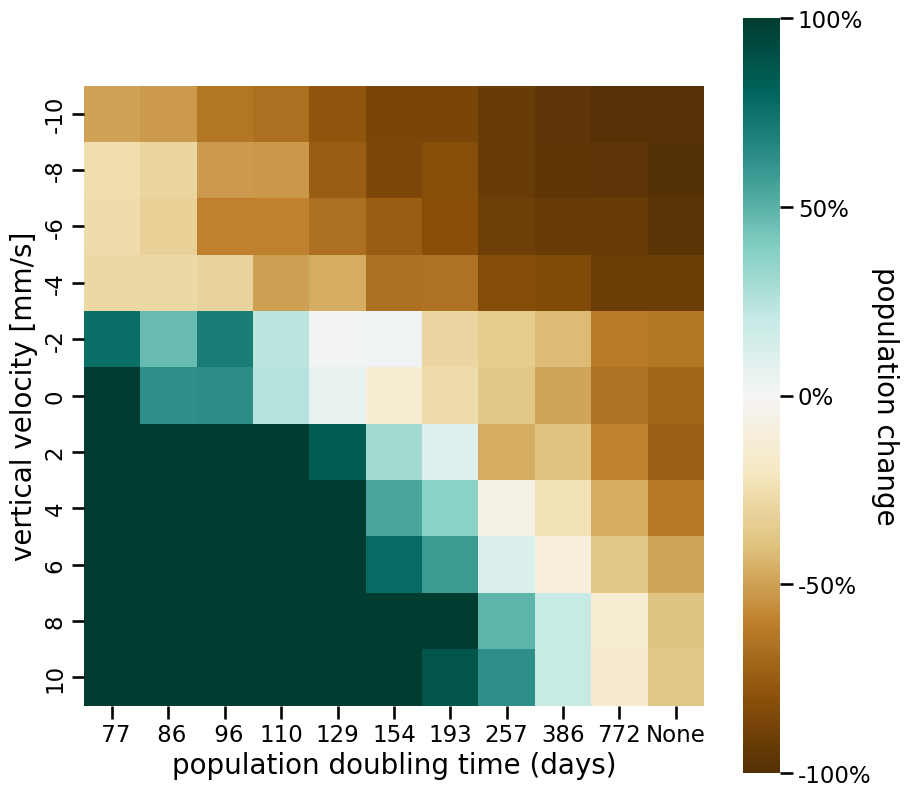
\includegraphics[width=\columnwidth]{diel_success.png}
    \caption[]{total particles counts for scenario "migration" with a monotonic migration pattern for all tested parameters}
    \label{fig:monotonic_particle_counts}
\end{figure}
% \begin{figure}
%     \includegraphics[width=\columnwidth]{example-image-a}
%     \caption[]{total particles counts for scenario "migration" with a diel migration pattern for all tested parameters}
%     \label{fig:diel_particle_counts}
% \end{figure}

In fig \ref{fig:dust_particle_counts} the particle counts measured over time it the estuary are shown.
We can clearly see that the total particle count drops to zero - in most cases already after less then two months.
From this we deduce that particles are constantly getting washed out and do not find "sheltered areas" 
in which they can remain for a long time.
This also means that reproduction is a necessary condition for the population to maintain their size 
even if all mortality sources except high-salinity are ignored.

In fig \ref{fig:monotonic_particle_counts} and \ref{fig:diel_particle_counts} we can see 
that the population manages to maintain themselves in certain conditions.
The fact that we found conditions for survival in this simplistic setup is in itself interesting for two major reasons.
First, all previsous studies implementing a phytoplankton in an Elbe model required constant reseeding either up and/or downstream.
Hence, we are the first study that is able to provide an estimate for the conditions necessary for "in-estuar"-survival.
\texttt{ The secondly might be better suited for the discussion.}
Secondly, while we assume ad libitum nutrient conditions for the phytoplankton we do not implement any sub-grid-resolution structure on the shores.
Hence, the river banks are perfectly flat sand banks without vegetation which might aid the retention of phytoplankton.

\texttt{Add comparison of monotonic upwards to downwards, monotonic to diel, and the discuss the relative growth rate thresholds}

Taking a closer look at the subset of pytoplankton that was able to retain themselves compared to those getting washed out.
You can see these measurement visualized in the boxplots \ref{fig:migration-long-vs-short}

\begin{figure}
    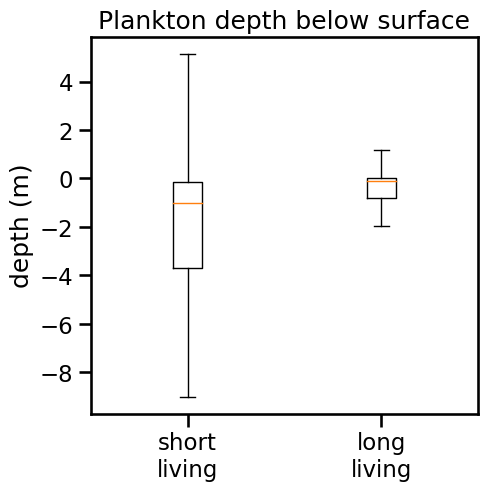
\includegraphics[width=\columnwidth]{dbf_bar.png}
    \caption[]{Boxplot of long-vs-short showing water depth}
    \label{fig:migration-long-vs-short}
\end{figure}

We can consistently see that the long living subset is in shallower water, does move less, and is a significantly longer stranded then drifting.
In fig. \ref{fig:migration-long-vs-short-heatmap} we show the special distribution of the long- and short-living subset
 also indication their predominance of long living phytoplankton close to the shores and in side channels.

\begin{figure}
    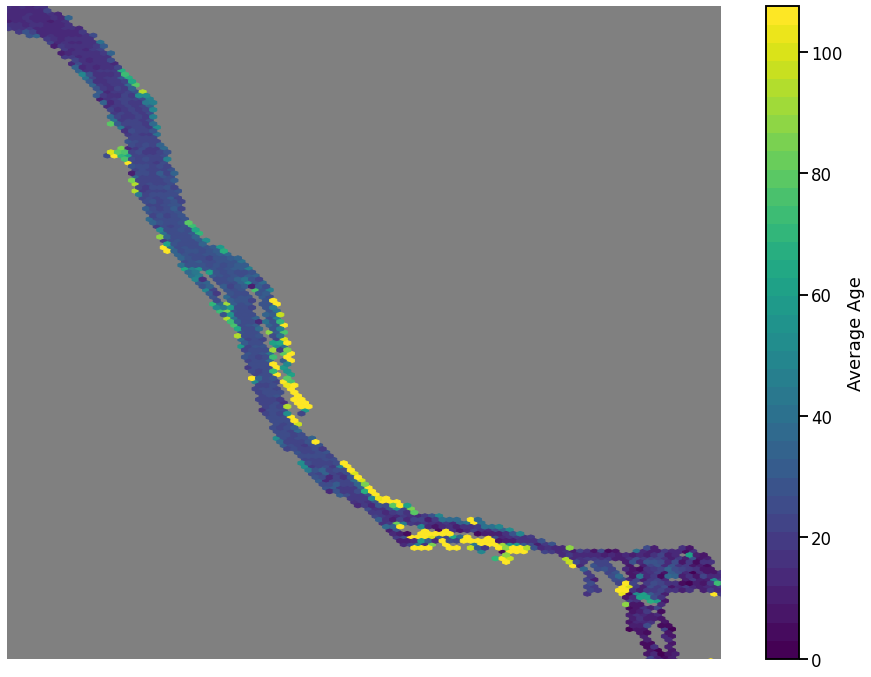
\includegraphics[width=\columnwidth]{heatmap.png}
    \caption[]{heatmap of long-living to short-living-particles}
    \label{fig:migration-long-vs-short-heatmap}
\end{figure}

\texttt{show zoom in with water depth?}

\subsubsection*{Scenario: "ready-for-liftoff"}

\begin{figure}
    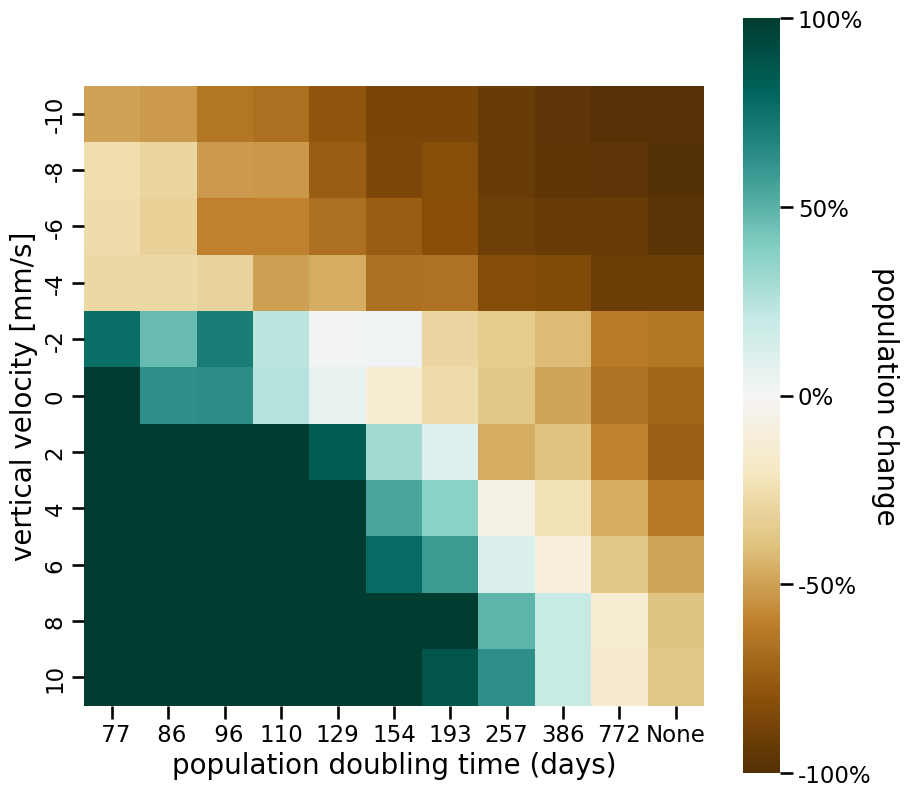
\includegraphics[width=\columnwidth]{diel_success.png}
    \caption[]{total particles counts for scenario "ready-for-liftoff" with a monotonic migration pattern for all tested parameters}
    \label{fig:stranded-monotonic-particle-counts}
\end{figure}

In fig \ref{fig:stranded-monotonic-particle-counts} we again show the total particle counts.
Keep in mind that the only difference in the model configuration to the "migration" run is that phytoplankton growth has been disabled when the plankton is stranded.
We can clearly see that phytoplankton dies out in these conditions for the full parameter space.
From this we deduce that the shallow areas are not only crucial for improved retention but also a necessary hatching ground.

To summarize the retention experiments: We saw that the population is ultimately washed out and perishes if we suppress reproduction.
We also saw that reproducing phytoplankton is able to maintain their population strain without up- or downstream reseeding under certain conditions!
We further showed that the shallow water areas are not only helpful for retention but crucial for the survival of the population.

\textbf{upstream migration}

% \highlight{I dropped this part for the time being.}
\begin{figure}
    \includegraphics[width=\columnwidth]{example-image-a}
    \caption[]{particle counts in upstream statistical polygons}
    \label{fig:upstream-migration-statistical-poly-counts}
\end{figure}


In the upstream migration experiment we divide the estuary in short ($\sim 50km$) sections.
We release particles in all of these sections and count their occurrence in other sections.
As previously described - in fig \ref{fig:upstream-migration-statistical-poly-counts} we see the 
the particle counts for the two upstream sections from the release location.
We consider upstream migration to happen when plankton moves two sections up and is able to retain itself there.
\texttt{Do I need to explain why two polygons and why being there only briefly won't work?}

\texttt{No results yet with the proper dispersion model. 
        In the previous run upstream migration did not occur and was considered 
        to be a negligible mechanism in the retention process.
        However, this might chance with the enabling of tidal pumping mechanisms.}


\section*{Discussion}

\subsection*{Interpretation and contextualization of Results}

\begin{itemize}
    \item retention success threshold as a measure of estimating outwashing losses
    \item very low outwashing rates imply unfavorable conditions for phytoplankton? or maybe the conditions are good and they grow nicely but not enough to compensate for losses in harbor?
    \item 
\end{itemize}



\subsection*{Limitations of the model}

\texttt{The discussion is currently only a list of bullet points that I considered to discuss so far. It is by no means complete or currently not worth reading.}
\begin{itemize}
    \item discuss limitation of the model
    \begin{itemize}
        \item simplified bottom/sediment interaction
        \item no "small object" representation e.g. vegetation or "rocks" $\rightarrow$ implices underestimation of "retention"
        \item simplistic bio representation. does not allow for precise quantification but only indicates bounds aka "even in ideal conditions they couldn't survive if ..."
        \item other minor issues - temporal resolution, particle out-of-bounds cases etc
        \item discuss choice of particle tracking model compared to concentration based model
    \end{itemize}
    \item conclusions that we draw from this:
    \begin{itemize}
        \item from a population-surival perspective the plankton that does not drift to shallow water are "dead man walking" as all decendents of these particles will ultimately die.
        \item we need cross-shore sampling to better understand this. currently all specially resolved sampling strategies are along shor - aka in the center of the river
        \item shallow water is crucial for the survival. hence the protection and restoration of shallow regions is crucial for ecosystem healthiness
    \end{itemize}
\end{itemize}

\bibliography{references.bib}
\bibliographystyle{unsrt}

\end{document}




